% COMPILER: pdfLaTeX
\documentclass[12pt,a4paper,twoside,openright]{book}

\usepackage[a4paper,twoside,width=150mm,top=30mm,bottom=30mm,bindingoffset=6mm]{geometry}
\usepackage[utf8]{inputenc}
\usepackage[T1]{fontenc}
\usepackage[italian]{babel}
\usepackage{caption}
\usepackage{parskip}
\usepackage[printonlyused,withpage]{acronym}
\usepackage[hidelinks]{hyperref}
\usepackage{emptypage}
\usepackage{ragged2e}
\usepackage{amsmath}
\usepackage{graphicx}
\usepackage[svgnames]{xcolor}
\usepackage[nocheck]{fancyhdr}
\usepackage{fancyvrb}
\usepackage{titlesec}
\usepackage{minted}
\usepackage[nottoc]{tocbibind}
\usepackage{csquotes}
\usepackage[sorting=none]{biblatex}

% Metadata setup
\hypersetup{
    pdftitle={Sviluppo di un'infrastruttura virtuale per l'erogazione di servizi di calcolo con SLURM},
    pdfsubject={Tesi di Laurea in Amministrazione di Sistemi T - CdS in Ingegneria Informatica},
    pdfauthor={Massimo Valerio Zerbini},
    pdfkeywords={HPC, SLURM, Vagrant, Ansible, IaC, Git, QoS, Federazione, Networking}
}

% Bibliography setup
\addbibresource{bibliografia.bib}
\setlength\bibitemsep{0.6\baselineskip}

% Chapter title style 
\titleformat{\chapter}[hang]{\Huge\bfseries}{\thechapter\hspace{20pt}\textcolor{Silver}{|}\hspace{20pt}}{0pt}{\Huge\bfseries}

% Page style modifications
\renewcommand{\chaptermark}[1]{\markboth{#1}{}}
\renewcommand{\tocetcmark}[1]{\markboth{#1}{}}
\renewcommand{\sectionmark}[1]{\markright{\thesection\quad #1}}
\fancyhf{}
\fancyhead[LE,RO]{\bfseries\thepage}
\fancyhead[LO]{\sl\bfseries\rightmark}
\fancyhead[RE]{\sl\bfseries\leftmark}
\renewcommand{\headrulewidth}{0.5pt}
\fancypagestyle{plain}{
    \fancyhead{}
    \renewcommand{\headrulewidth}{0pt}
}

% Minted default document-wide style
\setminted{style=default,frame=lines,framesep=2mm,framerule=0.3pt,rulecolor=darkgray,baselinestretch=1.2,bgcolor=WhiteSmoke,fontsize=\footnotesize,linenos,breaklines,highlightcolor=LemonChiffon}
% Minted language-specific styles
\setminted[properties]{style=sas}
\setminted[console]{linenos=false,frame=leftline}
\setminted[yaml]{escapeinside=||}


\pagestyle{fancy}


\begin{document} % ===============================================================
\begin{titlepage}
\newgeometry{centering}
\begin{center}
{{\Large{\textsc{Alma Mater Studiorum $\cdot$ Universit\`a di Bologna}}}}
\rule[0.1cm]{\linewidth}{0.1mm}
\rule[0.5cm]{\linewidth}{0.6mm}\\
\vspace{3mm}
{\small{\bf Scuola di Ingegneria e Architettura\\ 
Dipartimento di Informatica -- Scienza e Ingegneria (DISI)\\
Corso di Laurea in Ingegneria Informatica}}\\
\vspace{10mm}
Tesi di Laurea in:\\
\textbf{Amministrazione di Sistemi T}
\end{center}
\vspace{21mm}
\begin{center}
{\large \bf SVILUPPO DI UN'INFRASTRUTTURA VIRTUALE\\[1mm] PER L'EROGAZIONE DI SERVIZI DI CALCOLO\\[1mm] CON SLURM\par}
\end{center}
\vspace{32mm}
\begin{minipage}[t]{0.45\textwidth}{
\large{
Relatore:
\vspace{2mm}\\{
\bf Prof. Marco Prandini
}
\vspace{6mm}\\{
Correlatore:
\vspace{2mm}\\
\bf Ing. Andrea Giovine
}
}}
\end{minipage}
\hfill
\begin{minipage}[t]{0.45\textwidth}\raggedleft{
{\large{Presentata da:\\
\vspace{2mm}
\bf Massimo Valerio Zerbini}}}
\end{minipage}
\vspace{32mm}
\begin{center}
Appello V\\
\vspace{1mm}
Anno Accademico 2023/2024
\end{center}
\end{titlepage}
\restoregeometry

\cleardoublepage
\begin{flushright}
\thispagestyle{empty}
\null\vspace{\stretch {1}}
\textit{
    ``It is only when they go wrong, that machines\break remind you how powerful they are.''\\
    \vspace{1.5mm} --- Clive James}
\vspace{\stretch{2}}\null
\end{flushright}

\chapter*\phantomsection
\thispagestyle{empty}
\begin{center}
\textbf{\large Abstract}\\
\vspace{1cm}
\begin{minipage}{13cm}
\begin{justify}
Nel presente elaborato di tesi viene descritto e analizzato il processo di sviluppo di un'infrastruttura virtuale \acs{SLURM}, per l'integrazione di specifici servizi di calcolo in ambito \acfi{HPC}. In particolare, si implementano la condivisione delle risorse di computazione, la definizione di una priorità di \textit{scheduling} e la federazione di due \textit{cluster} virtuali. La progettazione dell'ambiente avviene applicando il principio di \acfi{IaC}, tramite strumenti come Vagrant e Ansible. Durante il processo di sviluppo, si affrontano e analizzano le varie difficoltà legate alla corretta configurazione dell'intera infrastruttura distribuita. Le funzionalità integrate vengono infine convalidate tramite l'esecuzione di test mirati.
\end{justify}
\end{minipage}
\end{center}

\tableofcontents


\chapter{Introduzione}\phantomsection % =========================================
Il contesto dell'\acf{HPC} rappresenta l'avanguardia per la risoluzione di problemi complessi e computazionalmente avanzati. Esso consiste nel coordinamento di più unità di elaborazione (raggruppate in ``\textit{cluster}'') per fornire esecuzioni ad alte prestazioni, ricorrendo tipicamente al calcolo simultaneo~\cite{hpcwikipedia}. La nascita del primo standard di programmazione parallela risale al 1990, ma in tempi recenti la potenza di calcolo ha raggiunto ordini di grandezza significativi per la simulazione di scenari reali.

L'applicazione di ambienti \ac{HPC} viene principalmente associata all'ambito della ricerca scientifica, ma il suo utilizzo è esteso a qualunque disciplina che necessiti di calcolo a elevate prestazioni; alcuni esempi sono:
\begin{itemize}
    \item la riproduzione e lo studio del clima globale (Climatologia);
    \item la risoluzione di equazioni fluidodinamiche (Fisica);
    \item la ricerca di metodi di conservazione per antichi testi e scritture (Archeologia);
    \item lo studio delle proteine per la cura di malattie degenerative (Medicina).
\end{itemize}
La progettazione e la manutenzione di un ambiente \ac{HPC} coinvolgono tecnologie e aspetti tipici dell'ingegneria informatica, tra cui l'amministrazione di sistemi. È infatti di cruciale importanza la corretta impostazione della comunicazione tra i diversi nodi interessati.

In questo elaborato di tesi viene descritto e analizzato il procedimento di sviluppo di un'infrastruttura virtuale distribuita, dedicata all'implementazione di diverse funzionalità inerenti al contesto \ac{HPC}. In particolare, verranno integrate:
\begin{itemize}
    \item la \textbf{condivisione delle risorse di computazione} disponibili, al fine di raggiungere il pieno utilizzo della potenza di calcolo;
    \item la \textbf{priorità di \textit{scheduling}} nei confronti di un determinato utente, ristretta a una specifica risorsa di computazione;
    \item la \textbf{federazione di \textit{cluster}}, ossia il coordinamento tra molteplici installazioni autonome per l'esecuzione di calcoli.
\end{itemize}

In primo luogo, si introdurranno le tecnologie e i particolari strumenti scelti per l'implementazione, discutendone il funzionamento e l'architettura.

In seguito, verrà progettato e definito l'ambiente virtuale \ac{IaC}, affrontando problematiche come la configurazione di rete, la risoluzione \acs{DNS} e la registrazione delle attività in un \acl{DB}.

In ultimo, verranno condotti test mirati per la verifica di ciascuna delle funzionalità implementate.


\chapter{Stato dell'arte} % ======================================================
\section{Virtualizzazione}
Una \acf{VM} (in italiano, \textit{macchina virtuale}) rappresenta un'emulazione virtuale di un calcolatore, ottenuta tramite astrazione delle risorse hardware della macchina ``\textit{host}'' (processo di virtualizzazione)~\cite{virtualizationwiki}. Esistono diversi tipi di virtualizzazione:
\begin{itemize}
    \item \textbf{Virtualizzazione nativa (o totale):} l'hardware viene completamente virtualizzato grazie all'uso di \textit{hypervisor} (figura \ref{fig:full-virtualization});
    \item \textbf{Virtualizzazione non nativa:} l'emulazione a livello software è basata su hardware diverso da quello fisicamente utilizzato, e necessita di codice aggiuntivo di basso livello per la compatibilità;
    \item \textbf{Paravirtualizzazione:} non viene simulato hardware in modo diretto, ma viene offerta una speciale \ac{API} per l'interazione tra macchine virtuali e risorse fisiche;
    \item \textbf{Containerizzazione:} implementa la virtualizzazione a livello di \textit{kernel} del sistema operativo, permettendo l'esecuzione contemporanea e isolata di istanze \textit{user-space}, senza \textit{overhead} dovuto all'emulazione hardware.
\end{itemize}
\begin{figure}[ht]
    \centering
    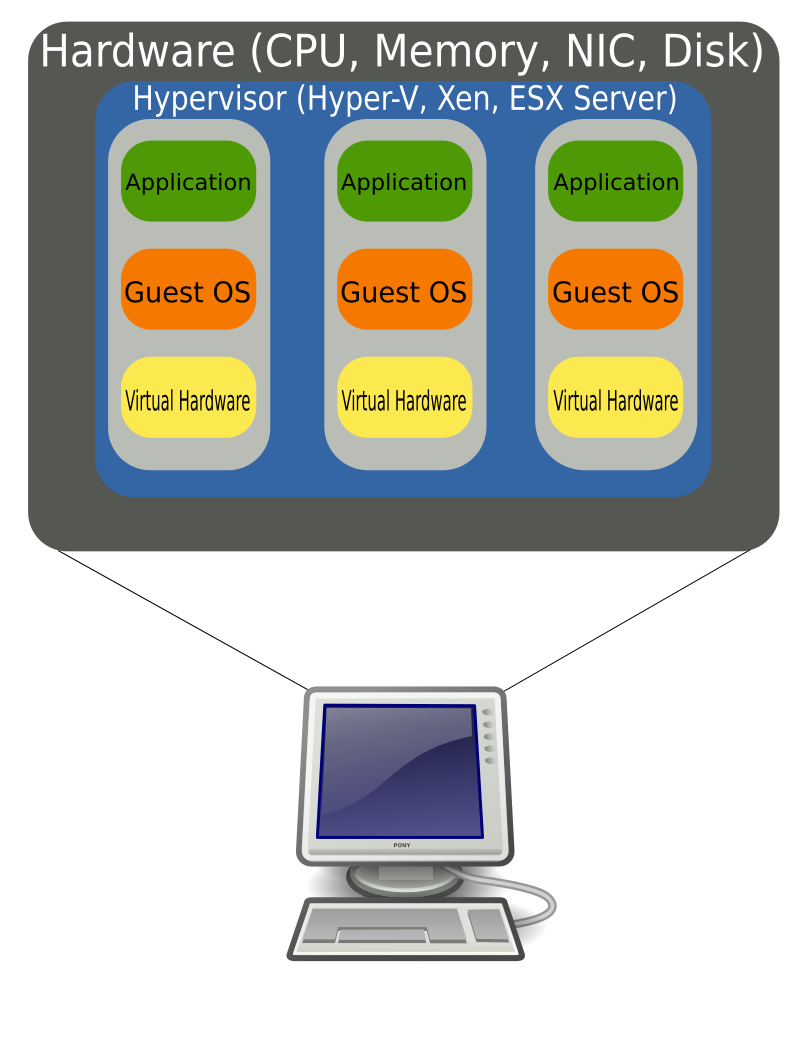
\includegraphics[width=0.5\linewidth]{images/full_virtualization.png}
    \caption{Virtualizzazione hardware totale~\cite{virtualizationwiki}}
    \label{fig:full-virtualization}
\end{figure}

Ciascun tipo di virtualizzazione offre un diverso equilibrio tra flessibilità e prestazioni; in particolare, la virtualizzazione totale si è dimostrata specialmente adatta per:
\begin{itemize}
    \item la condivisione di un sistema tra diversi utenti;
    \item l'isolamento dei programmi (e degli utenti) presenti sulle \ac{VM};
    \item l'emulazione di nuovo hardware per il raggiungimento di affidabilità, produttività e sicurezza.
\end{itemize}

\subsection{Vagrant}
Vagrant è un software \textit{open source} per la gestione di \ac{VM}, focalizzato sulla riproducibilità affidabile degli ambienti virtualizzati~\cite{vagrantwiki}. Nasce nel 2010 come progetto personale di Mitchell Hashimoto, ma cresce in popolarità dopo la fondazione di HashiCorp nel 2012.

\subsubsection{Architettura}
Vagrant dipende da software di virtualizzazione esterni (detti ``\textit{provider}'' o ``\textit{hypervisor}'') come VirtualBox\footnote{\url{https://www.virtualbox.org/}} e VMware\footnote{\url{https://www.vmware.com/}}, ma grazie al suo alto livello di astrazione, risulta portabile rispetto a essi.

Immagini di \ac{VM} di base (denominate ``\textit{box}'') sono facilmente reperibili e condivisibili su depositi online: ciò rappresenta un punto di forza per Vagrant, che solleva gli sviluppatori dal laborioso processo di inizializzazione degli ambienti virtuali. L'uso della virtualizzazione hardware permette l'esecuzione di ambienti e sistemi operativi indipendenti dalla macchina \textit{host}.

A tempo di esecuzione, Vagrant utilizza un file di configurazione (\texttt{Vagrantfile}) per ottenere i parametri definiti, quali immagine di base, specifiche hardware, cartelle condivise e indirizzi di rete locali.

\section{Provisioning}
Il \textit{provisioning} rappresenta l'insieme delle azioni preparatorie necessarie a rendere un sistema o servizio pienamente operativo~\cite{provisioningwiki}. Nell'ambito dell'amministrazione di sistemi, esempi tipici sono installazione/aggiornamento di software, configurazione di rete e gestione degli utenti.

\subsection{Ansible}
Ansible è un pacchetto di strumenti software \textit{open source} per la configurazione e gestione automatizzata di ambienti informatici, tramite file di definizione (principio noto come \acf{IaC})~\cite{ansiblewiki}~\cite{iacwiki}. Ansible nasce nel 2012 e viene acquisito dalla nota compagnia software RedHat nel 2015; è stato inizialmente sviluppato per sistemi Unix-like, ma ha esteso il proprio supporto anche a nodi Windows. Ansible è compatibile con computer fisici, macchine virtuali e interi ambienti \textit{cloud}.

\subsubsection{Architettura}
Ansible si basa su interazione ``\textit{agentless}'', dove il controllore, mediante una semplice connessione \acf{SSH}, esegue le operazioni definite sui nodi interessati, senza quindi l'esigenza di particolare software sul sistema destinatario (escludendo il server \ac{SSH}).

I nodi da gestire sono identificati tramite ``\textit{inventory}'', un file di testo che li elenca e li raggruppa. Per definire le operazioni da eseguire, Ansible utilizza i ``\textit{playbook}'', file descritti in linguaggio \ac{YAML} di semplice interpretazione.

L'elenco dei moduli responsabili delle azioni sui nodi è costantemente aggiornato e consultabile nella documentazione ufficiale~\cite{ansibledoc}. Essi sono sviluppati aspirando a un'alta astrazione dal sistema destinatario e all'idempotenza delle singole operazioni.

\section{DNS \& DHCP}
Il protocollo \acf{DNS} nasce in seguito all'esigenza di collegare indirizzi \ac{IP} a nomi di host, facilmente interpretabili e memorizzabili dagli esseri umani~\cite{dnswiki}. Per ciascuna zona di autorità è presente almeno un \textit{name server}, dove vengono mantenute le corrispondenze tra \textit{hostname} e indirizzi di competenza del dominio.

La risoluzione \ac{DNS} è un procedimento trasparente alle applicazioni e agli utenti finali. La richiesta di traduzione del nome di host viene trasmessa al \textit{resolver} locale, il quale ne controlla la presenza in memoria \textit{cache}; in caso di non disponibilità del record, la richiesta viene inoltrata in autonomia ai \textit{resolver} di livello superiore (figura \ref{fig:dns-resolution}).
\begin{figure}[ht]
    \centering
    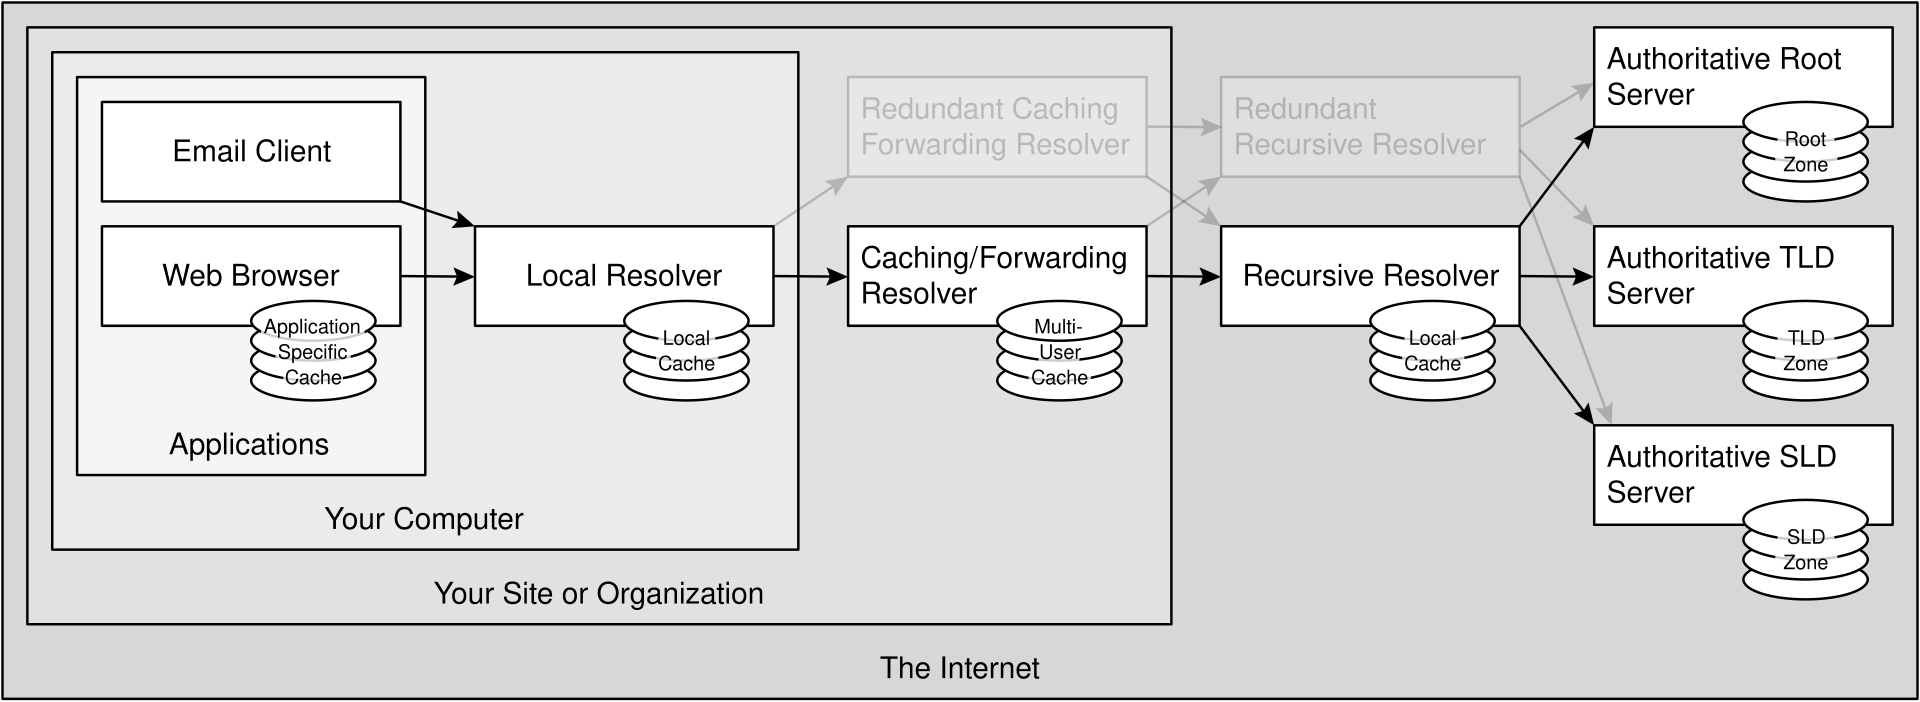
\includegraphics[width=0.95\linewidth]{images/dns_resolution.png}
    \caption{Sequenza di risoluzione \ac{DNS}~\cite{dnswiki}}
    \label{fig:dns-resolution}
\end{figure}

Il protocollo \acf{DHCP} svolge invece la funzione di assegnamento automatico e dinamico di indirizzi \ac{IP}, nell'ambito di una \ac{LAN}~\cite{dhcpwiki}.

\ac{DHCP} lavora in architettura \textit{client}/\textit{server}: al momento della connessione alla rete locale, il cliente invia una richiesta in \textit{broadcast}, e il server \ac{DHCP} di competenza risponde assegnando un indirizzo \ac{IP} locale all'interno di un intervallo configurabile.

\subsection{dnsmasq}
\texttt{dnsmasq} è un software \textit{open source} leggero e facilmente configurabile, in grado di fornire servizi \ac{DNS}/\ac{DHCP} su piccola scala~\cite{dnsmasqwiki}.

In caso di richieste di risoluzione \ac{DNS}, \texttt{dnsmasq} accede alla \textit{cache} locale ed eventualmente inoltra l'operazione a un effettivo \textit{resolver} ricorsivo. Per richieste \ac{DHCP}, \texttt{dnsmasq} si affida invece alla configurazione locale per allocazioni statiche o dinamiche. Il servizio \ac{DHCP} si integra in modo naturale con il servizio \ac{DNS}, consentendo la registrazione automatica delle corrispondenze \textit{hostname}/\textit{address} in seguito al \textit{leasing} degli indirizzi.

\section{Base di dati}
Un \acf{DB} (in italiano, \textit{base di dati}) è una collezione organizzata di dati accessibili tramite un \acf{DBMS}, un software di interfacciamento per amministratori, applicazioni e utenti finali~\cite{dbwiki}.

L'interazione con il \ac{DB} è regolata da linguaggi specializzati:
\begin{itemize}
    \item \acf{DCL} per il controllo dell'accesso ai dati;
    \item \acf{DDL} per la definizione di dati e delle relazioni tra di essi;
    \item \acf{DML} per la manipolazione dei dati (inserimento, modifica, rimozione);
    \item \acf{DQL} per la ricerca di informazioni estrapolate dai dati.
\end{itemize}
\acf{SQL} raggruppa le funzionalità di \ac{DDL}, \ac{DML} e \ac{DQL} in un singolo linguaggio, rappresentando uno standard \textit{de facto} nell'ambito delle basi di dati.

Le tipologie dominanti di \ac{DB} sono:
\begin{itemize}
    \item \textbf{Relazionale:} i dati sono strutturati in \textit{tabelle} collegate univocamente tra loro tramite \textit{relazioni} e \textit{chiavi} identificative (figura \ref{fig:relational-key}); ciascuna tabella simboleggia un'entità: le colonne indicano gli \textit{attributi}, mentre le righe rappresentano le sue \textit{istanze}; grazie alle \textit{transazioni}, i dati godono delle proprietà di \acf{ACID};
    \item \textbf{\acf{NoSQL}:} estensione dei \ac{DB} relazionali, con supporto verso ulteriori strutture (chiave:valore, documenti, colonne, grafi, ...); è indicato per applicazioni a bassa latenza ed elevato \textit{throughput}.
\end{itemize}
\begin{figure}[ht]
    \centering
    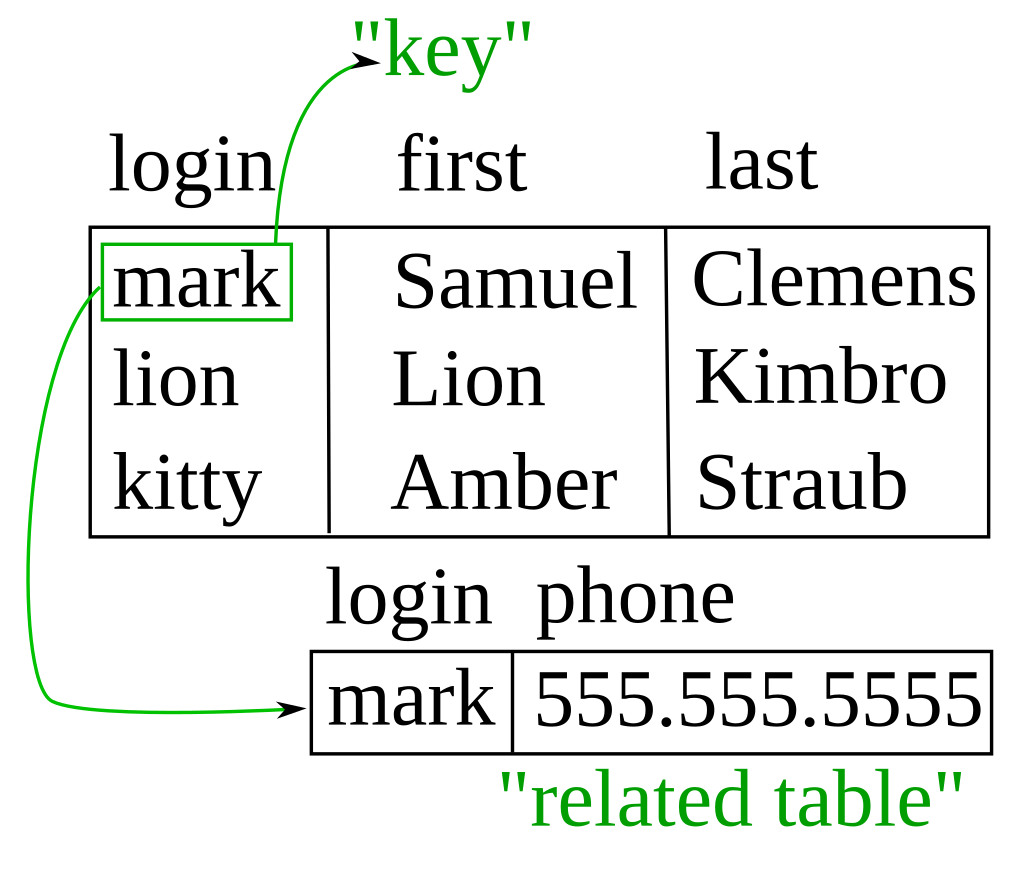
\includegraphics[width=0.35\linewidth]{images/relational_key.png}
    \caption{Modello relazionale~\cite{dbwiki}}
    \label{fig:relational-key}
\end{figure}

\subsection{MariaDB}
Maria\acs{DB} è un \ac{DBMS} relazionale \textit{open source}, basato sul diffuso My\ac{SQL}, con il quale aspira a mantenere un'alta compatibilità nonostante l'introduzione di funzionalità avanzate, come nuovi \textit{storage engine}~\cite{mariadbwiki}.

\section{Workload Management}
Il concetto di \textit{job scheduling} nasce con l'avvento dei primi sistemi informatici, in grado di eseguire una coda di schede perforate descriventi sequenze di istruzioni macchina~\cite{jobschedwiki}. I software moderni per la gestione di job sono tipicamente strutturati in architettura distribuita \textit{master}/\textit{agent}, con un singolo nodo di controllo e numerosi nodi di esecuzione.

\subsection{SLURM}
\acf{SLURM} è un software \textit{open source} per la gestione e il coordinamento di nodi di calcolo, finalizzato alla pianificazione e l'esecuzione di programmi (``\textit{jobs}'')~\cite{slurmoverview}. \ac{SLURM} è altamente scalabile, rendendolo adatto anche in contesti \acf{HPC} a intenso utilizzo di risorse.

Vengono integrate tre funzioni principali:
\begin{itemize}
    \item allocazione esclusiva (e non) delle risorse computazionali, per un periodo di tempo configurabile;
    \item inclusione di un \textit{framework} per la sottomissione e il monitoraggio dell'esecuzione di programmi;
    \item gestione della contesa di risorse mediante code di esecuzione.
\end{itemize}
È possibile includere funzionalità aggiuntive, quali registrazione delle attività (``\textit{accounting}'') e limitazione dell'uso di risorse, tramite il caricamento di \textit{plugin} opzionali.

\subsubsection{Architettura}
Come illustrato in figura \ref{fig:slurm-architecture}, un \textit{cluster} \ac{SLURM} è coordinato dal demone controllore \texttt{slurmctld}, il cui compito è gestire le richieste di esecuzione e allocare le risorse disponibili. Ciascun nodo di calcolo esegue \texttt{slurmd} per comunicare con il controllore ed effettuare i task richiesti. Il demone \texttt{slurmdbd}, connesso a un \ac{DBMS}, diventa essenziale per la registrazione delle attività di molteplici cluster in un singolo \ac{DB}; con esso vengono configurati gli \textit{account} per il controllo degli utenti abilitati alla sottomissione di programmi. È inoltre possibile raggruppare i nodi di computazione in partizioni logiche assestanti e configurabili individualmente.
\begin{figure}[ht]
    \centering
    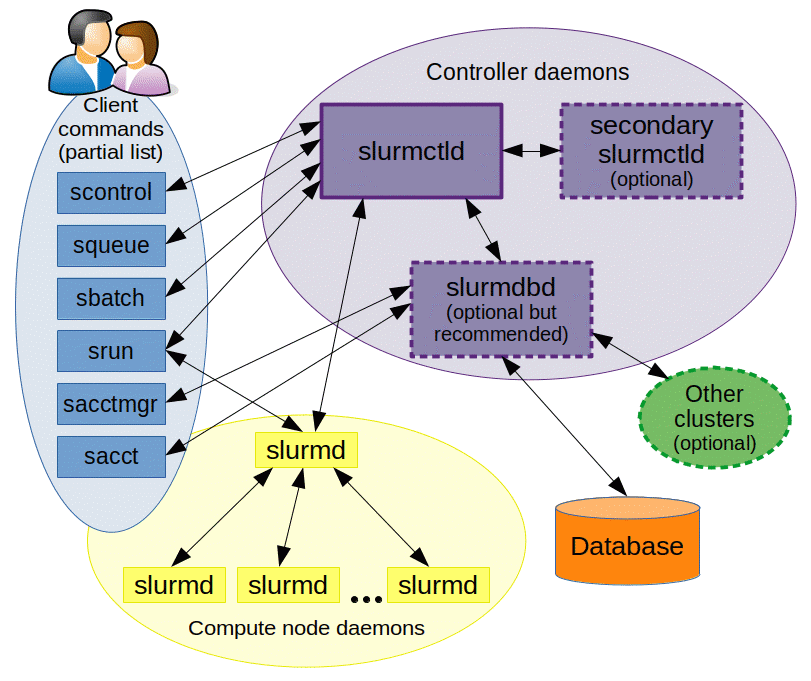
\includegraphics[width=0.65\linewidth]{images/slurm_architecture.png}
    \caption{Componenti di un cluster \ac{SLURM}~\cite{slurmoverview}}
    \label{fig:slurm-architecture}
\end{figure}

\subsubsection{Autenticazione}
Le interazioni tra i vari demoni \ac{SLURM} avvengono tramite \acf{RPC}: è dunque necessario verificare l'autenticità della fonte del messaggio. Di default si utilizza \acf{MUNGE}, un servizio per la creazione e validazione di credenziali utente, progettato appositamente per ambienti \ac{HPC}~\cite{slurmauth}.

La codifica/decodifica delle credenziali si basa su una chiave comune, condivisa ai soli nodi fidati. Un prerequisito fondamentale per il corretto funzionamento di \ac{MUNGE} è la coerenza di utenti e gruppi in tutti i nodi interessati~\cite{mungedoc}.

\subsubsection{Condivisione di risorse}
Di default, \ac{SLURM} alloca in modo esclusivo interi nodi di computazione per l'esecuzione dei programmi: ciò significa che, anche in caso di basso utilizzo di risorse, nessun altro job verrà inoltrato allo stesso nodo. Per superare l'inefficienza di questo scenario, è possibile attivare la condivisione di risorse, quali \ac{CPU} e \ac{RAM}~\cite{slurmconstres}; configurazioni più granulari sono applicabili per le componenti della \ac{CPU}, come \textit{socket} e \textit{core} (figura \ref{fig:slurm-cpu-cores}).
\begin{figure}[ht]
    \centering
    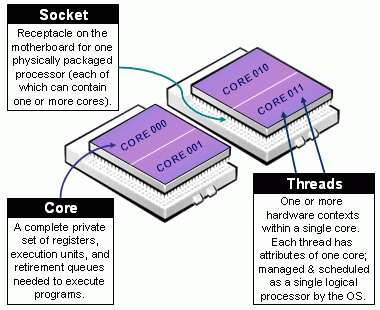
\includegraphics[width=0.6\linewidth]{images/cpu_cores_sockets_threads.png}
    \caption{Definizioni di \textit{socket}, \textit{core} e \textit{thread}~\cite{slurmcpucore}}
    \label{fig:slurm-cpu-cores}
\end{figure}

Ulteriori tipologie di risorse, come le \ac{GPU}, vengono supportate sotto la classificazione di \acf{GRES}: per esse è necessaria la precisa definizione tramite file di configurazione. È inoltre possibile la loro condivisione tra i diversi job in coda~\cite{slurmgres}.

\subsubsection{Priorità di scheduling}
\ac{SLURM} offre numerosi metodi per impostare la priorità di \textit{scheduling} tra i job; i principali sono:
\begin{itemize}
    \item configurazione del \textbf{peso di molteplici fattori} (``\textit{Multifactor Priority}'') per la selezione del job da eseguire, come ad esempio la sua dimensione, la quantità di risorse richieste e il tempo trascorso in coda~\cite{slurmmultifactor};
    \item definizione di \textbf{\acf{QoS}} per partizioni o singoli nodi~\cite{slurmqos}, con la possibilità di limitare l'uso di risorse specifiche~\cite{slurmlimits}.
\end{itemize}

\subsubsection{Federazione}
\ac{SLURM} permette la definizione di federazioni di \textit{cluster}, dove la sottomissione dei job è inoltrata a tutti i componenti~\cite{slurmfederation}. Ciascuno di essi tenta dunque di portare a termine la richiesta di esecuzione, in modo indipendente. Per il corretto coordinamento all'interno della federazione, è necessario che tutte le istanze di \texttt{slurmctld} (una per cluster) possano comunicare tra loro, oltre che con la singola istanza di \texttt{slurmdbd}, dedicata alla registrazione delle attività (figura \ref{fig:slurm-federation}).
\begin{figure}[ht]
    \centering
    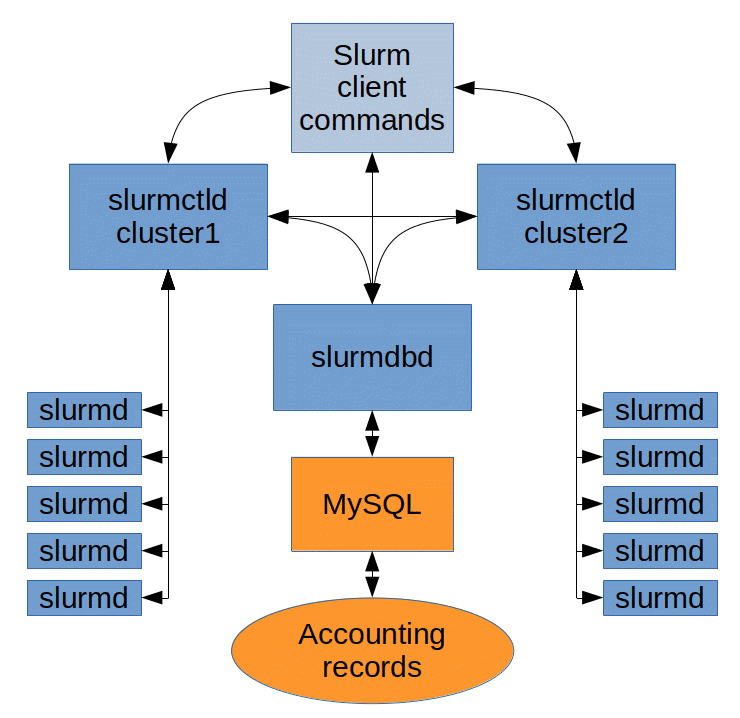
\includegraphics[width=0.55\linewidth]{images/slurm_federation.png}
    \caption{Comunicazione in una federazione \ac{SLURM}~\cite{slurmnetwork}}
    \label{fig:slurm-federation}
\end{figure}


\chapter{Analisi progettuale} % ==================================================
Il progetto si pone di sviluppare, in stile \acf{IaC}, un'infrastruttura di \ac{VM} dedicata all'integrazione di particolari funzionalità \ac{SLURM}. Di seguito sono analizzati i passi necessari.

\subsubsection{Macchine virtuali}
L'implementazione richiede anzitutto la scelta di un \textit{hypervisor} (in grado di fornire virtualizzazione totale) e di una \textit{box} Vagrant di riferimento; si è dunque optato per VirtualBox\footnote{\url{https://www.virtualbox.org/}}, nativamente supportato da Vagrant, e Debian Bookworm\footnote{\url{https://www.debian.org/releases/bookworm/}}, un sistema operativo basato su Linux e noto per la sua stabilità ed efficienza.

Una funzionalità interessante di VirtualBox sono le \textit{linked clone}~\cite{linkedclone}, macchine virtuali basate sulle differenze con il disco della \textit{box} di base, al fine di evitarne la copia totale (figura \ref{fig:linked-clone}). In questo modo, l'\textit{overhead} dovuto alla creazione di molteplici \ac{VM} viene ridotto al minimo.
\begin{figure}[ht]
    \centering
    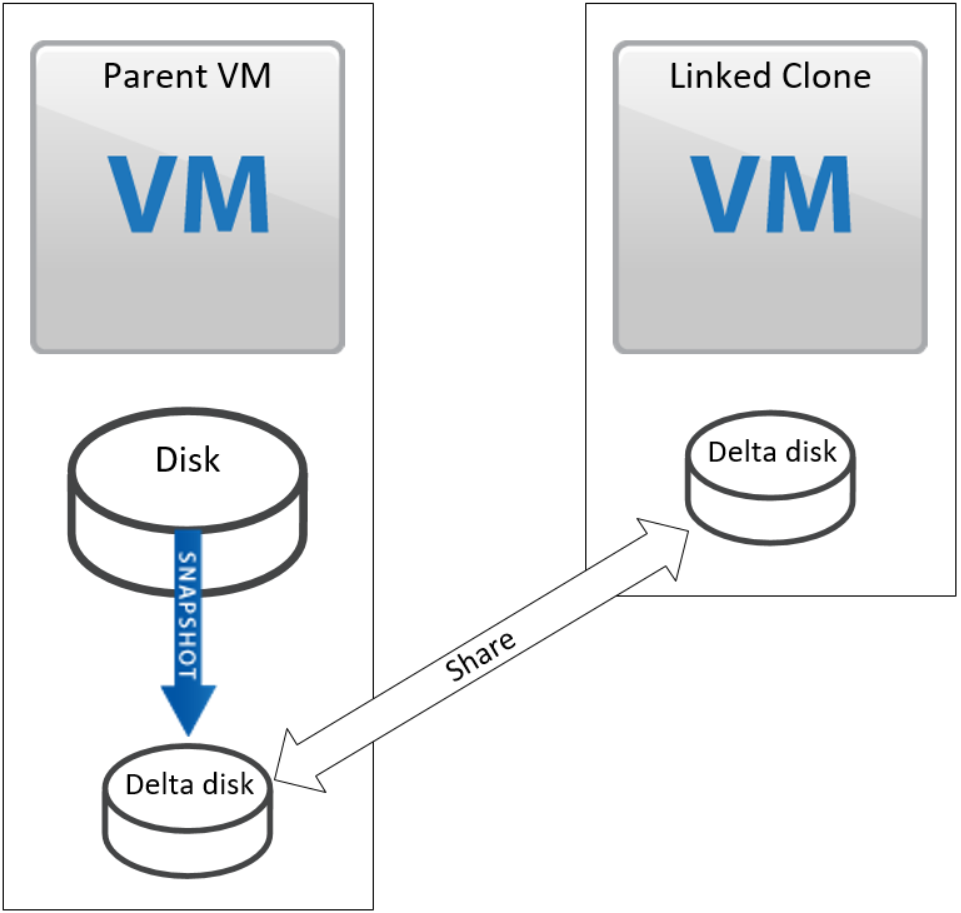
\includegraphics[width=0.5\linewidth]{images/linked_clone.png}
    \caption{Relazione tra \ac{VM} di base e \textit{linked clone}~\cite{clonetypes}}
    \label{fig:linked-clone}
\end{figure}

Il \textit{provisioning} delle macchine virtuali viene svolto da diversi \textit{playbook} Ansible.

\subsubsection{DHCP \& DNS}
\ac{SLURM} basa le proprie comunicazioni su nomi di host, astraendo da indirizzi \ac{IP}; è quindi necessaria la corretta risoluzione \ac{DNS} all'interno della \ac{LAN}. La scelta di \texttt{dnsmasq} offre inoltre funzionalità \ac{DHCP} per più reti.

\subsubsection{Accounting}
Essendo prevista la registrazione delle attività (``\textit{accounting}'') in ambienti multi-cluster \ac{SLURM}, è necessaria la configurazione di un \ac{DB} e relativo \ac{DBMS}; è stato scelto Maria\acs{DB} per familiarità con il contesto \ac{SQL}. L'interazione tra il \ac{DBMS} e il demone \texttt{slurmdbd}, responsabile dell'\textit{accounting}, è configurabile seguendo la documentazione appropriata~\cite{slurmaccounting}.

\subsubsection{Topologia di rete}
Una federazione \ac{SLURM}, per definizione, è composta da più \textit{cluster} in coordinamento tra loro; in contesti concreti, è verosimile che ciascuno di essi sia confinato nella propria \ac{LAN}, dove la trasmissione verso l'esterno viene mediata da un \textit{router} (o \textit{gateway}). La figura \ref{fig:topology} visualizza la topologia di rete per due \textit{cluster} in federazione.
\begin{figure}[ht]
    \centering
    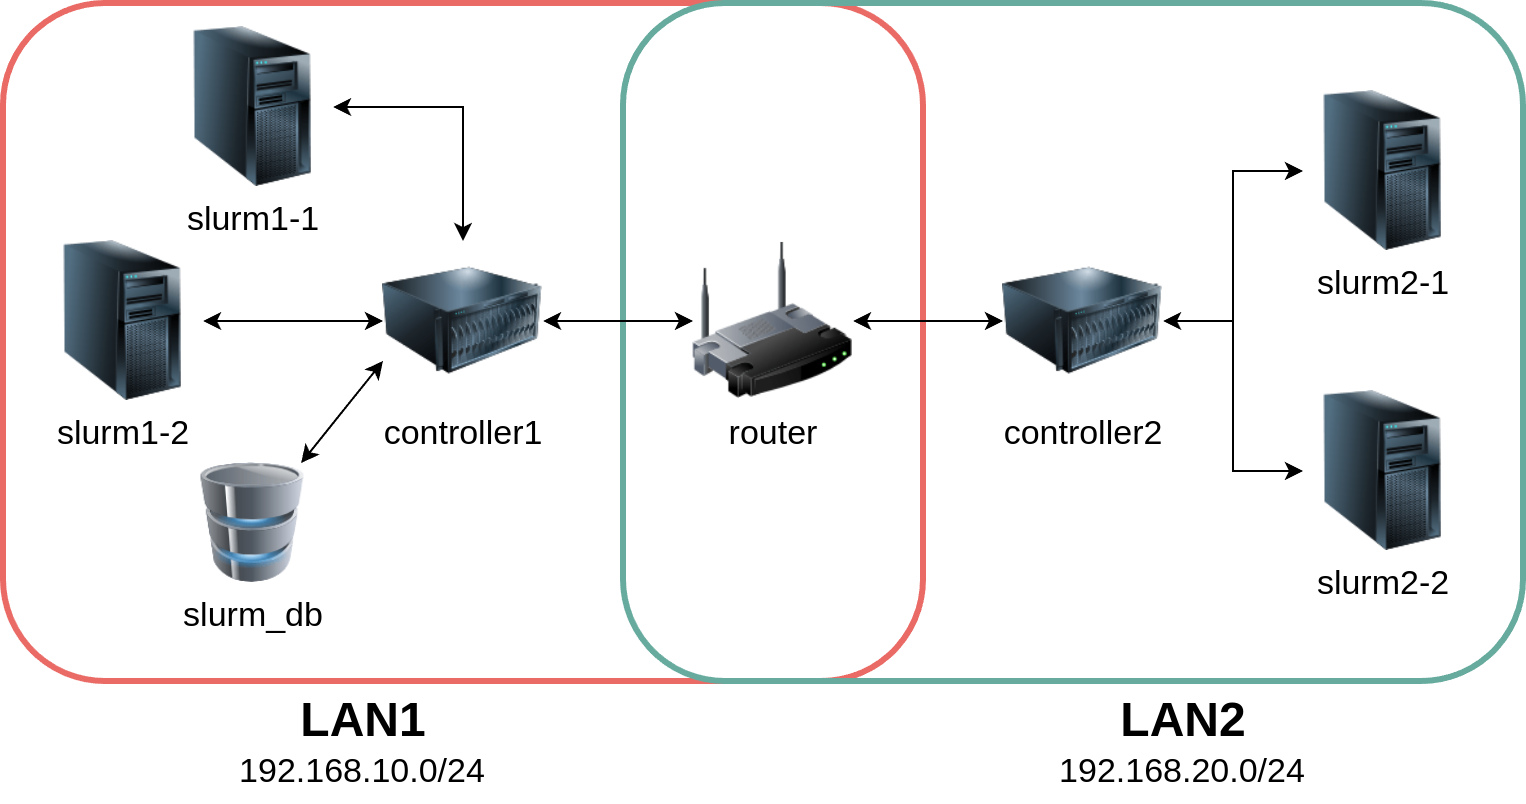
\includegraphics[width=0.9\linewidth]{images/topology.png}
    \caption{Topologia virtuale desiderata}
    \label{fig:topology}
\end{figure}

In particolare, la configurazione della macchina virtuale \texttt{router} deve permettere la corretta comunicazione tra le due reti, inoltrando i pacchetti interessati.

\subsubsection{Condivisione di risorse}
La condivisione delle risorse disponibili su un nodo è configurabile grazie al \textit{plugin} \texttt{select/cons\_tres}~\cite{slurmconstres}. Il progetto si pone, nello specifico, la condivisione di \ac{CPU}, \ac{RAM} e \ac{GPU}; essendo quest'ultima catalogata come \acf{GRES}, è necessaria una configurazione aggiuntiva per il corretto interfacciamento~\cite{slurmgres}.

\subsubsection{Priorità di scheduling}
Una volta attiva la condivisione di risorse, si può impostare la priorità di \textit{scheduling}, ottenuta grazie alla definizione di una partizione \ac{SLURM} separata e all'utilizzo del \textit{plugin} \texttt{priority/multifactor}~\cite{slurmmultifactor}.

Sulla partizione viene applicata una \acf{QoS} prioritaria~\cite{slurmqos}, accessibile dall'utente desiderato e ristretta a una singola \ac{GPU} del nodo di computazione~\cite{slurmlimits}.

\subsubsection{Federazione di cluster}
Ciascun \textit{cluster} \ac{SLURM} è descritto interamente da un proprio file di configurazione, che deve essere coerente su tutti i suoi nodi. Per la generazione di due installazioni, è dunque necessario definire due file separati, da inoltrare correttamente alle rispettive macchine virtuali.

Una prerogativa essenziale per l'impostazione di una federazione \ac{SLURM} è la registrazione, sullo stesso \ac{DB}, di tutti i cluster coinvolti, tramite l'uso di una singola istanza di \texttt{slurmdbd}~\cite{slurmfederation}.


\chapter{Implementazione} % ======================================================
L'intero codice sviluppato per l'implementazione è consultabile pubblicamente su un \textit{repository} Git\footnote{\url{https://github.com/maxzrbn/Tirocinio-SLURM}}.

\section{Infrastruttura}
\subsection{Macchine virtuali}
Il primo passo è la definizione delle macchine virtuali, seguendo il grafico e la nomenclatura presentati in figura \ref{fig:topology}; è necessario prestare attenzione ai seguenti aspetti:
\begin{itemize}
    \item creazione delle \ac{VM} come \textit{linked clone} della \textit{box} di base;
    \item corretto assegnamento delle reti interne VirtualBox (\texttt{LAN1} e \texttt{LAN2});
    \item delega del \textit{provisioning} a un \textit{playbook} Ansible.
\end{itemize}
Il file di definizione Vagrant risulta così composto:
\begin{minted}[label=Vagrantfile]{ruby}
Vagrant.configure("2") do |config|
  #
  # VM BOX CONFIGURATION
  config.vm.box = "debian/bookworm64"
  config.vm.provider "virtualbox" do |vb|
    vb.linked_clone = true
    vb.memory = "1024"
    vb.cpus = "4"
  end
  #
  # VIRTUAL MACHINES
  config.vm.define "router" do |machine|
    machine.vm.hostname = "router"
    machine.vm.network "private_network", virtualbox__intnet: "LAN1", auto_config: false
    machine.vm.network "private_network", virtualbox__intnet: "LAN2", auto_config: false
  end
  (1..2).each do |i|
    config.vm.define "controller#{i}" do |machine|
      machine.vm.hostname = "controller#{i}"
      machine.vm.network "private_network", virtualbox__intnet: "LAN#{i}", auto_config: false
    end
    (1..2).each do |j|
      config.vm.define "slurm#{i}-#{j}" do |machine|
        machine.vm.hostname = "slurm#{i}-#{j}"
        machine.vm.network "private_network", virtualbox__intnet: "LAN#{i}", auto_config: false
      end
    end
  end
  #
  # PROVISIONING
  config.vm.provision "ansible" do |ansible|
    ansible.playbook = "site.yml"
  end
end
\end{minted}
Ciascun nodo è quindi virtualmente dotato di 4 \ac{CPU} e 1 \ac{GB} di \ac{RAM}. Da notare l'uso di iterazioni per la definizione compatta di molteplici \ac{VM}.

Il \textit{provisioning} Ansible viene definito in \texttt{site.yml}, attribuendo ``ruoli'' alle varie macchine virtuali; ciascuno di essi esegue una particolare sequenza di istruzioni.
\begin{minted}[label=site.yml]{yaml}
---
- hosts: router
  become: true
  roles:
    - common
    - router

- hosts: controller1
  become: true
  roles:
    - common
    - mariadb
    - slurmcommon
    - cluster1
    - slurmctlr

- hosts: controller2
  become: true
  roles:
    - common
    - slurmcommon
    - cluster2
    - slurmctlr

- hosts: slurm1-1:slurm1-2
  become: true
  roles:
    - common
    - slurmcommon
    - cluster1
    - slurmwkr

- hosts: slurm2-1:slurm2-2
  become: true
  roles:
    - common
    - slurmcommon
    - cluster2
    - slurmwkr
\end{minted}

\subsection{Configurazione di rete}
Svolgendo la funzione di \ac{DHCP}/\ac{DNS} server, la macchina virtuale \texttt{router} dispone di due interfacce di rete con indirizzi \ac{IP} locali statici; è possibile configurarle grazie al seguente file, opportunamente inoltrato alla \ac{VM}:
\begin{minted}[label=roles/router/files/eth\_cfg]{properties}
auto eth1
iface eth1 inet static
  netmask 255.255.255.0
  address 192.168.10.254

auto eth2
iface eth2 inet static
  netmask 255.255.255.0
  address 192.168.20.254
\end{minted}
Affinché si possano effettivamente instradare i pacchetti tra le due \ac{LAN}, è necessario attivare, su \texttt{router}, il \textit{forwarding} a livello di \textit{kernel}, modificando un particolare file di configurazione:
\begin{minted}[label=roles/router/tasks/main.yml]{yaml}
|\textcolor{black}{...}|
- name: Allow IPv4 forwarding
  ansible.builtin.lineinfile:
    path: '/etc/sysctl.conf'
    line: 'net.ipv4.ip_forward=1'
    state: present
  notify: Reload kernel config
|\textcolor{black}{...}|
\end{minted}
Le interfacce delle restanti \ac{VM} vengono automaticamente configurate grazie al protocollo \ac{DHCP}.

\subsection{DHCP \& DNS}
Il servizio \ac{DHCP}/\ac{DNS} è svolto, per entrambe le reti, da \texttt{dnsmasq}, in esecuzione su \texttt{router}. La sua configurazione è la seguente:
\begin{minted}[label=roles/router/files/dnsmasq.conf,highlightlines=21]{properties}
interface=eth1
interface=eth2
no-hosts
no-resolv

# NAMESERVER USED FOR THE INTERNET (the host running the VMs)
server=10.0.2.3

# ADDRESS RANGES FOR LEASING
dhcp-range=interface:eth1,192.168.10.1,192.168.10.253,12h
dhcp-range=interface:eth2,192.168.20.1,192.168.20.253,12h

# SPECIFY SELF AS NAMESERVER (for both LANs)
dhcp-option-force=interface:eth1,option:dns-server,192.168.10.254
dhcp-option-force=interface:eth2,option:dns-server,192.168.20.254

# AVOID ROUTING ALL TRAFFIC THROUGH THIS VM
dhcp-option=3

# STATIC ROUTE FOR CROSS-LAN COMMUNICATION
dhcp-option=121,192.168.20.0/24,192.168.10.254,192.168.10.0/24,192.168.20.254
\end{minted}
L'opzione evidenziata specifica il \textit{gateway} tra le reti, ossia l'instradamento dei pacchetti provenienti da una \ac{LAN} e destinati all'altra.

\subsection{Accounting}
La registrazione delle attività (``\textit{accounting}'') viene svolta dal demone \texttt{slurmdbd}, in esecuzione su \texttt{controller1}.

\subsubsection{Database}
Per integrare l'inserimento di password nel \textit{provisioning}, si definiscono apposite variabili di esecuzione, eventualmente crittografabili con l'ausilio di Ansible Vault~\cite{ansibledoc}:
\begin{minted}[label=secrets.yml]{yaml}
mariadb:
  root_password: THIS_IS_THE_ROOT_DB_PASSWORD
  slurm_password: THIS_IS_THE_SLURM_DB_PASSWORD
\end{minted}
Al fine di isolare l'installazione del \ac{DB}, si può utilizzare il software di containerizzazione \texttt{podman}\footnote{\url{https://podman.io/}}, in grado di recuperare ed eseguire l'immagine di Maria\acs{DB} opportunamente configurata:
\begin{minted}[label=roles/mariadb/tasks/main.yml]{yaml}
|\textcolor{black}{...}|
- name: Pull a MariaDB container
  become: true
  become_user: 'mariadb'
  containers.podman.podman_image:
    name: 'mariadb:latest'

- name: Run MariaDB container
  become: true
  become_user: 'mariadb'
  containers.podman.podman_container:
    name: 'mariadb'
    image: 'mariadb:latest'
    state: started
    ports: "127.0.0.1:3306:3306"
    env:
        MARIADB_ROOT_PASSWORD: "{{ mariadb.root_password }}"
|\textcolor{black}{...}|
\end{minted}
In questo modo Maria\acs{DB} risulta in ascolto sulla porta \ac{TCP} \texttt{3306} di \texttt{controller1}.

Seguendo poi la documentazione \ac{SLURM} per il corretto interfacciamento tra il \ac{DBMS} e \texttt{slurmdbd}~\cite{slurmaccounting}, si generano \ac{DB} e utente dedicati:
\begin{minted}[label=roles/mariadb/tasks/main.yml]{yaml}
|\textcolor{black}{...}|
- name: Ensure 'slurm_db' database is present
  community.mysql.mysql_db:
    name: slurm_db
    state: present
    login_host: 127.0.0.1
    login_port: 3306
    login_user: root
    login_password: "{{ mariadb.root_password }}"
  retries: 6
  delay: 10

- name: Ensure 'slurm' MySQL user is present with password
  community.mysql.mysql_user:
    name: slurm
    password: "{{ mariadb.slurm_password }}"
    host: '%'
    login_host: 127.0.0.1
    login_user: root
    login_password: "{{ mariadb.root_password }}"
    state: present
|\textcolor{black}{...}|
\end{minted}
Si impostano poi i privilegi appropriati, assicurandosi che vengano salvati e applicati (operazione di ``\textit{flushing}''):
\begin{minted}[label=roles/mariadb/tasks/main.yml]{yaml}
|\textcolor{black}{...}|
- name: Grant usage privilege to the user
  community.mysql.mysql_user:
    name: slurm
    priv: '*.*:USAGE'
    append_privs: yes
    host: '%'
    login_host: 127.0.0.1
    login_user: root
    login_password: "{{ mariadb.root_password }}"
    state: present

- name: Grant all privileges on the database to the user
  community.mysql.mysql_user:
    name: slurm
    priv: 'slurm_db.*:ALL'
    append_privs: yes
    host: '%'
    login_host: 127.0.0.1
    login_user: root
    login_password: "{{ mariadb.root_password }}"
    state: present

- name: Flush privileges (update & reload grant tables)
  community.mysql.mysql_user:
    login_user: root
    login_password: "{{ mariadb.root_password }}"
    check_implicit_admin: yes
    append_privs: yes
    login_host: 127.0.0.1
    state: present
    name: slurm
    host: '%'
|\textcolor{black}{...}|
\end{minted}
A questo punto è possibile verificare manualmente l'accesso al \ac{DB}, presentandosi come utente \texttt{slurm} (utilizzato poi da \texttt{slurmdbd}):
\begin{minted}{console}
vagrant@controller1:~$ mariadb -u slurm --port=3306 --password=THIS_IS_THE_SLURM_DB_PASSWORD slurm_db
Reading table information for completion of table and column names
You can turn off this feature to get a quicker startup with -A

Welcome to the MariaDB monitor.  Commands end with ; or \g.
Your MariaDB connection id is 12
Server version: 11.5.2-MariaDB-ubu2404 mariadb.org binary distribution

Copyright (c) 2000, 2018, Oracle, MariaDB Corporation Ab and others.

Type 'help;' or '\h' for help. Type '\c' to clear the current input statement.

MariaDB [slurm_db]>_
\end{minted}

\subsubsection{slurmdbd}
Si prosegue con l'installazione del demone \texttt{slurmdbd}:
\begin{minted}[label=roles/mariadb/tasks/main.yml]{yaml}
|\textcolor{black}{...}|
- name: Install 'slurmdb' package
  ansible.builtin.apt:
    name: 'slurmdbd'
    update_cache: true
|\textcolor{black}{...}|
\end{minted}
Il suo file di configurazione è così composto:
\begin{minted}[label=slurmdbd.conf]{properties}
AuthType=auth/munge
DbdHost=controller1
DbdPort=6819
DebugLevel=verbose
StorageHost=localhost
StorageLoc=slurm_db
StoragePass="{{ mariadb.slurm_password }}"
StoragePort=3306
StorageType=accounting_storage/mysql
StorageUser=slurm
LogFile=/var/log/slurm/slurmdbd.log
PidFile=/run/slurmdbd.pid
SlurmUser=slurm
\end{minted}
Da notare le opzioni:
\begin{itemize}
    \item \mintinline{properties}{AuthType=auth/munge}: attivazione del \textit{plugin} \ac{MUNGE} per l'autenticazione delle trasmissioni \ac{RPC};
    \item \mintinline{properties}{DbdPort=6819}: porta \ac{TCP} di ascolto per le comunicazioni con gli altri componenti \ac{SLURM}.
\end{itemize}

Nel tentativo di avviare il demone si sono però presentati i seguenti errori:
\begin{minted}[highlightlines=4]{console}
vagrant@controller1:~$ sudo slurmdbd -D -vvv
slurmdbd: debug2: accounting_storage/as_mysql: init: mysql_connect() called for db slurm_db
slurmdbd: debug2: Attempting to connect to localhost:3306
slurmdbd: error: mysql_real_connect failed: 2002 Can't connect to local server through socket '/run/mysqld/mysqld.sock' (2)
slurmdbd: error: The database must be up when starting the MYSQL plugin.  Trying again in 5 seconds.
\end{minted}
Indagando sul messaggio evidenziato si è appreso che \texttt{slurmdbd}, specificata l'opzione \mintinline{properties}{StorageHost=localhost}, tenta la connessione al \ac{DB} tramite \textit{socket} locale di default (\texttt{/run/mysqld/mysqld.sock})~\cite{slurmaccounting}; eseguendo però il \ac{DBMS} all'interno di un \textit{container}, la posizione della \textit{socket} diventa relativa al \textit{filesystem} astratto:
\begin{minted}[breakanywhere]{console}
vagrant@controller1:~$ sudo find / -type s | grep 'mysqld.sock'
/home/mariadb/.local/share/containers/storage/overlay/e7d63d4ddde910afaf1d2574c3345fc74c42372bffc95f84528ead29c2f52d7e/diff/run/mysqld/mysqld.sock
\end{minted}
È dunque necessario aggiornare il file di configurazione con \mintinline{properties}{StorageHost=127.0.0.1}, in modo da forzare il demone all'utilizzo di porte \ac{TCP}/\ac{IP}.

\subsection{Cluster SLURM}
\label{clusterconf}
Il file di configurazione \texttt{slurm.conf} viene utilizzato da entrambi \texttt{slurmctld} e \texttt{slurmd}; in esso è descritto il generico comportamento del \textit{cluster}:
\begin{minted}[label=roles/cluster1/templates/slurm.conf,highlightlines=24]{properties}
# CLUSTER 1 CONFIG
#
ClusterName=cluster1
SlurmctldHost=controller1
MpiDefault=none
ProctrackType=proctrack/cgroup
ReturnToService=1
SlurmctldPidFile=/var/run/slurmctld.pid
SlurmctldPort=6817
SlurmdPidFile=/var/run/slurmd.pid
SlurmdPort=6818
SlurmdSpoolDir=/var/slurm/slurmd
SlurmUser=slurm
SlurmdUser=root
StateSaveLocation=/var/slurm/slurmctld
SwitchType=switch/none
TaskPlugin=task/affinity
#
# SCHEDULING
SchedulerType=sched/backfill
SelectType=select/linear
#
# LOGGING AND ACCOUNTING
AccountingStorageType=accounting_storage/slurmdbd
AccountingStorageUser=slurm
JobAcctGatherType=jobacct_gather/cgroup
SlurmctldLogFile=/var/log/slurm/slurmctld.log
SlurmdLogFile=/var/log/slurm/slurmd.log
#
# COMPUTE NODES
NodeName=slurm1-[1-2] CPUs=4 State=UNKNOWN
PartitionName=debug Nodes=ALL Default=YES MaxTime=INFINITE State=UP
\end{minted}
Con l'opzione evidenziata, \texttt{slurmctld} attiva e delega la registrazione delle attività a \texttt{slurmdbd}, in esecuzione sul medesimo nodo (\texttt{controller1}).

La configurazione del secondo \textit{cluster} presenta invece alcune differenze:
\begin{minted}[label=roles/cluster2/templates/slurm.conf,highlightlines=6]{properties}
# CLUSTER 2 CONFIG
#
ClusterName=cluster2
SlurmctldHost=controller2
...
AccountingStorageHost=controller1
...
NodeName=slurm2-[1-2] ...
...
\end{minted}
L'opzione in evidenza, specificata solo nel \textit{cluster} senza \ac{DB}, indica il nodo da contattare per l'\textit{accounting} delle attività, dove viene eseguito \texttt{slurmdbd}.

\section{Condivisione di risorse}
Per la condivisione delle risorse è necessario modificare opportunamente i file di configurazione; di seguito vengono indicate le variazioni relative al primo \textit{cluster}, ma le differenze con il secondo interessano esclusivamente la nomenclatura dei nodi:
\begin{minted}[label=roles/cluster1/templates/slurm.conf]{properties}
...
SelectType=select/cons_tres
SelectTypeParameters=CR_CPU_Memory
...
AccountingStorageTRES=gres/gpu
...
GresTypes=gpu
NodeName=slurm1-[1-2] CPUs=4 RealMemory=1024 Gres=gpu:rtx2080ti:2 State=UNKNOWN
...
\end{minted}
In particolare, le opzioni indicano~\cite{slurmconstres}:
\begin{itemize}
    \item \mintinline{properties}{SelectType=select/cons_tres}: \textit{plugin} per la gestione delle risorse (``\textit{consumable trackable resources}''), permettendo l'esecuzione di più job sullo stesso nodo;
    \item \mintinline{properties}{SelectTypeParameters=CR_CPU_Memory}: risorse ordinarie da condividere (nel caso in questione, \ac{CPU} e \ac{RAM});
    \item \mintinline{properties}{AccountingStorageTRES=gres/gpu}: attivazione dell'\textit{accounting} relativo alle \ac{GPU};
    \item \mintinline{properties}{GresTypes=gpu}: tipologie di \acf{GRES} da condividere;
    \item \mintinline{properties}{RealMemory=1024}: memoria totale in \ac{MB} allocabile per nodo di computazione (opzione obbligatoria per la condivisione della memoria; deve essere minore o uguale alla \ac{RAM} riconosciuta dal sistema operativo);
    \item \mintinline{properties}{Gres=gpu:rtx2080ti:2}: specifiche \ac{GRES} presenti nel nodo.
\end{itemize}
È inoltre fondamentale introdurre nei nodi di computazione due ulteriori file di configurazione, per il corretto interfacciamento con le \ac{GRES}~\cite{slurmgres}:
\begin{minted}[label=roles/slurmwkr/templates/cgroup.conf]{properties}
CgroupPlugin=autodetect
CgroupAutomount=yes
ConstrainCores=no
ConstrainRAMSpace=no
ConstrainDevices=yes
\end{minted}
In \texttt{gres.conf} vanno specificati:
\begin{itemize}
    \item il nome del nodo di computazione;
    \item le precise caratteristiche delle risorse presenti.
\end{itemize}
\begin{minted}[label=gres.conf]{properties}
NodeName=slurm1-1 Name=gpu Type=rtx2080ti Count=2 File=/dev/nvidia[0-1]
\end{minted}
Una volta configurate, è possibile verificare la disponibilità delle risorse tramite il comando \texttt{sinfo}:
\begin{minted}{console}
vagrant@controller1:~$ sinfo -o "%15N  %10c  %10m  %20G"
NODELIST         CPUS        MEMORY      GRES
slurm1-[1-2]     4           1024        gpu:rtx2080ti:2
\end{minted}

\section{Priorità di scheduling}
L'applicazione di una priorità di \textit{scheduling} necessita anzitutto di un contesto verosimile di utilizzo; a tal proposito vengono definiti utenti/gruppi di prova, tra cui quelli interessati dalla priorità (in questo caso, \texttt{user1}).

Affinché venga mantenuta la coerenza di utenti/gruppi all'interno del \textit{cluster}, la loro definizione avviene con task comuni a tutti i nodi:
\begin{minted}[label=roles/slurmcommon/tasks/main.yml]{yaml}
|\textcolor{black}{...}|
- name: Ensure test groups exist
  ansible.builtin.group:
    name: "{{ item.name }}"
    gid: "{{ item.id }}"
    state: present
  loop:
    - { name: 'user1', id: '2001' }
    - { name: 'user2', id: '2002' }
    - { name: 'user3', id: '2003' }
    - { name: 'user4', id: '2004' }

- name: Ensure test users exist
  ansible.builtin.user:
    name: "{{ item.name }}"
    uid: "{{ item.id }}"
    group: "{{ item.name }}"
    state: present
  loop:
    - { name: 'user1', id: '2001' }
    - { name: 'user2', id: '2002' }
    - { name: 'user3', id: '2003' }
    - { name: 'user4', id: '2004' }
|\textcolor{black}{...}|
\end{minted}
Il file di configurazione \ac{SLURM} è stato modificato nel seguente modo:
\begin{minted}[label=roles/cluster1/templates/slurm.conf]{properties}
...
PriorityType=priority/multifactor
PriorityWeightQOS=10000
PriorityWeightTRES=GRES/gpu=100
...
AccountingStorageEnforce=limits
JobAcctGatherType=jobacct_gather/cgroup
...
PartitionName=gpupart Nodes=slurm1-[1-2] QOS=gpuprio AllowAccounts=user1acct State=UP
\end{minted}
In particolare, le opzioni specificano:
\begin{itemize}
    \item \mintinline{properties}{PriorityType=priority/multifactor}: \textit{plugin} per la priorità a molteplici fattori~\cite{slurmmultifactor}; per il caso in questione si sono privilegiate, tramite le opzioni\\ \texttt{PriorityWeight-}:
    \begin{itemize}
        \item l'appartenenza a \acf{QoS} prioritarie;
        \item la richiesta di \ac{GPU} per l'esecuzione;
    \end{itemize}
    \item \mintinline{properties}{AccountingStorageEnforce=limits}: imposizione dei limiti sulle risorse specificati nel \ac{DB}; implica la presenza di un'associazione (utente, account, partizione, ...) valida per tutte le richieste di esecuzione~\cite{slurmlimits};
    \item \mintinline{properties}{PartitionName=gpupart}: partizione aggiuntiva ristretta all'account \texttt{user1acct}, con \ac{QoS} \texttt{gpuprio} (definiti in seguito).
\end{itemize}

\subsection{Impostazione del DB}
È fondamentale la registrazione nel \ac{DB} (tramite il comando \texttt{sacctmgr}) delle informazioni per il comportamento desiderato, ovvero:
\begin{itemize}
    \item la \ac{QoS} \texttt{gpuprio}~\cite{slurmqos};
    \item gli account \texttt{user1acct} (prioritario) e \texttt{noprio}~\cite{slurmaccounting}.
\end{itemize}
\begin{minted}{console}
vagrant@controller1:~$ sudo sacctmgr add qos gpuprio Priority=10 GrpTRES=gres/gpu=1
 Adding QOS(s)
  gpuprio
 Settings
  Description    = gpuprio
  GrpTRES                  = gres/gpu=1
  Priority                 = 10
Would you like to commit changes? (You have 30 seconds to decide)
 (N/y): y
vagrant@controller1:~$ sudo sacctmgr add account user1acct QOS=gpuprio
 Adding Account(s)
  user1acct
 Settings
  Description     = Account Name
  Organization    = Parent/Account Name
 Associations =
  C = cluster1    A = user1acct
 Settings
  QOS           = gpuprio
Would you like to commit changes? (You have 30 seconds to decide)
 (N/y): y
vagrant@controller1:~$ sudo sacctmgr add account noprio
 Adding Account(s)
  noprio
 Settings
  Description     = Account Name
  Organization    = Parent/Account Name
 Associations =
  C = cluster1    A = noprio
Would you like to commit changes? (You have 30 seconds to decide)
 (N/y): y
\end{minted}
L'account \texttt{noprio} risulta essenziale affinché gli utenti non prioritari possano richiedere l'esecuzione di job. Da notare il confinamento della priorità a una singola \ac{GPU}, tramite l'attributo \texttt{GrpTRES}~\cite{slurmlimits}.

Gli utenti, durante la registrazione nel \ac{DB}, vengono collegati a un account di default, pertinente al comportamento desiderato:
\begin{minted}{console}
vagrant@controller1:~$ sudo sacctmgr add user user1 DefaultAccount=user1acct
 Adding User(s)
  user1
 Settings
  Default Account = user1acct
 Associations =
  C = cluster1    A = user1acct            U = user1
Would you like to commit changes? (You have 30 seconds to decide)
 (N/y): y
vagrant@controller1:~$ sudo sacctmgr add user user2,user3,user4 DefaultAccount=noprio
 Adding User(s)
  user2
  user3
  user4
 Settings
  Default Account = noprio
 Associations =
  C = cluster1    A = noprio               U = user2
  C = cluster1    A = noprio               U = user3
  C = cluster1    A = noprio               U = user4
Would you like to commit changes? (You have 30 seconds to decide)
 (N/y): y
\end{minted}
Il comando \texttt{sacctmgr} permette infine di verificare le informazioni registrate:
\begin{minted}{console}
vagrant@controller1:~$ sacctmgr show qos format=name,priority,GrpTRES
      Name   Priority       GrpTRES
---------- ---------- -------------
    normal          0              
   gpuprio         10    gres/gpu=1
vagrant@controller1:~$ sacctmgr show association user=user1,user2,user3,user4 format=user,account,qos
      User    Account                  QOS
---------- ---------- --------------------
     user2     noprio               normal
     user3     noprio               normal
     user4     noprio               normal
     user1  user1acct              gpuprio
\end{minted}

\section{Federazione di cluster}
L'implementazione di una federazione \ac{SLURM} si basa sulla corretta impostazione dei singoli \textit{cluster}, svolta in sezione \ref{clusterconf}.

La seguente opzione, non essenziale per il funzionamento in sé, imposta la visualizzazione federata per i comandi \texttt{sacctmgr} e \texttt{scontrol}~\cite{slurmfederation}:
\begin{minted}[label=roles/cluster1/templates/slurm.conf]{properties}
...
FederationParameters=fed_display
...
\end{minted}

\subsection{Impostazione del DB}
La registrazione di entrambi i \textit{cluster} sullo stesso \ac{DB} è un requisito fondamentale per l'impostazione della federazione~\cite{slurmfederation}:
\begin{minted}{console}
vagrant@controller1:~$ sudo sacctmgr add federation testfederation clusters=cluster1,cluster2
 Adding Federation(s)
  testfederation
 Settings
  Cluster       = cluster1
  Cluster       = cluster2
Would you like to commit changes? (You have 30 seconds to decide)
 (N/y): y
\end{minted}
Utilizzando \texttt{sacctmgr} e \texttt{scontrol}, si è dunque confermata la corretta comunicazione tra di essi:
\begin{minted}{console}
vagrant@controller1:~$ sacctmgr show federation
Federation    Cluster ID             Features     FedState
---------- ---------- -- -------------------- ------------
testfeder+   cluster1  1                            ACTIVE
testfeder+   cluster2  2                            ACTIVE
vagrant@controller1:~$ scontrol show federation
Federation: testfederation
Self:       cluster1:127.0.0.1:6817 ID:1 FedState:ACTIVE Features:
Sibling:    cluster2:192.168.20.194:6817 ID:2 FedState:ACTIVE Features: PersistConnSend/Recv:Yes/Yes Synced:Yes
\end{minted}


\chapter{Risultati} % ============================================================
L'accertamento della funzionalità dei servizi \ac{SLURM} proposti richiede, in primo luogo, l'avvio dell'intera infrastruttura. Tramite il comando ``\texttt{vagrant up}'', la creazione e il \textit{provisioning} delle macchine virtuali vengono automatizzati in stile \acf{IaC}.

Il comando \texttt{sinfo} convalida la disponibilità dei \textit{cluster} aderenti alla federazione:
\begin{minted}{console}
vagrant@controller1:~$ sinfo
PARTITION CLUSTER  AVAIL  TIMELIMIT  NODES  STATE NODELIST
debug*    cluster1    up   infinite      1   idle slurm1-[1-2]
debug*    cluster2    up   infinite      1   idle slurm2-[1-2]
\end{minted}

\section{Test della condivisione di risorse}
Per verificare la condivisione delle risorse presenti su un nodo, vengono allocati quattro job da 1 \ac{CPU} (\texttt{-c1}) e 256 \ac{MB} di \ac{RAM} (\texttt{{-}{-}mem=256}), specificandone lo svolgimento su un singolo nodo (\texttt{-N1}) da 4 \ac{CPU} e 1 \ac{GB} di \ac{RAM}:
\begin{minted}{console}
vagrant@controller1:~$ srun -N1 -c1 --mem=256 sleep 60 &
[1] 18254
vagrant@controller1:~$ srun -N1 -c1 --mem=256 sleep 60 &
[2] 18264
vagrant@controller1:~$ srun -N1 -c1 --mem=256 sleep 60 &
[3] 18274
vagrant@controller1:~$ srun -N1 -c1 --mem=256 sleep 60 &
[4] 18284
\end{minted}
Grazie al comando \texttt{squeue} è possibile confermare l'esecuzione contemporanea dei job (tutti in stato \textit{running}), a dimostrazione della condivisione di processori e memoria:
\begin{minted}{console}
vagrant@controller1:~$ squeue
JOBID PARTITION     NAME     USER ST       TIME  NODES NODELIST(REASON)
    1     debug    sleep  vagrant  R       0:15      1 slurm1-1
    2     debug    sleep  vagrant  R       0:14      1 slurm1-1
    3     debug    sleep  vagrant  R       0:13      1 slurm1-1
    4     debug    sleep  vagrant  R       0:12      1 slurm1-1
\end{minted}
Allo stesso modo, vengono allocati due job richiedenti 1 \ac{GPU} ciascuno (\texttt{{-}{-}gpus=1}) verificando la loro esecuzione parallela e quindi la condivisione delle \ac{GPU}:
\begin{minted}{console}
vagrant@controller1:~$ srun -N1 --gpus=1 --mem=256 sleep 60 &
[1] 18294
vagrant@controller1:~$ srun -N1 --gpus=1 --mem=256 sleep 60 &
[2] 18304
vagrant@controller1:~$ squeue
JOBID PARTITION     NAME     USER ST       TIME  NODES NODELIST(REASON)
    5     debug    sleep  vagrant  R       0:08      1 slurm1-1
    6     debug    sleep  vagrant  R       0:07      1 slurm1-1
\end{minted}

\section{Test della priorità di scheduling}
Per confermare la priorità di \textit{scheduling} su una \ac{GPU}, da parte di un determinato utente, vengono allocati tre job non prioritari e un job lanciato da \texttt{user1} (sulla partizione prioritaria \texttt{gpupart}):
\begin{minted}{console}
vagrant@controller1:~$ sudo -u user2 srun -N1 --gpus=1 --mem=256 sleep 60 &
[1] 18314
vagrant@controller1:~$ sudo -u user3 srun -N1 --gpus=1 --mem=256 sleep 60 &
[2] 18324
vagrant@controller1:~$ sudo -u user4 srun -N1 --gpus=1 --mem=256 sleep 60 &
[3] 18334
vagrant@controller1:~$ sudo -u user1 srun -N1 --partition=gpupart --gpus=1 --mem=256 sleep 60 &
[4] 18344
vagrant@controller1:~$ squeue
JOBID PARTITION     NAME     USER ST       TIME  NODES NODELIST(REASON)
    9     debug    sleep    user4 PD       0:00      1 (Resources)
    8     debug    sleep    user3  R       0:03      1 slurm1-1
    7     debug    sleep    user2  R       0:17      1 slurm1-1
   10   gpupart    sleep    user1 PD       0:00      1 (QOSGrpGRES)
\end{minted}
Il job \texttt{10} risulta quindi in concorrenza di risorse con il job \texttt{9} (entrambi in stato \textit{pending}). Attendendo la liberazione di una \ac{GPU} (ossia il termine del job \texttt{7}), la partizione prioritaria ha la precedenza di \textit{scheduling}:
\begin{minted}[highlightlines=5]{console}
vagrant@controller1:~$ squeue
JOBID PARTITION     NAME     USER ST       TIME  NODES NODELIST(REASON)
    9     debug    sleep    user4 PD       0:00      1 (Resources)
    8     debug    sleep    user3  R       0:50      1 slurm1-1
   10   gpupart    sleep    user1  R       0:04      1 slurm1-1
\end{minted}

\section{Test della federazione di cluster}
Grazie all'opzione \texttt{{-}{-}clusters} in fase di sottomissione, è possibile specificare una lista di \textit{cluster} sulla quale tentare di eseguire il job richiesto (ad esempio, il programma \texttt{hostname}):
\begin{minted}{console}
vagrant@controller1:~$ srun --clusters=cluster2 -N2 hostname
slurm2-1
slurm2-2

vagrant@controller2:~$ srun --clusters=cluster1 -N2 hostname
slurm1-1
slurm1-2
\end{minted}
È importante notare come, per entrambe le sottomissioni di esempio:
\begin{itemize}
    \item il controllore di partenza non appartenga al \textit{cluster} specificato per l'esecuzione;
    \item venga richiesta l'esecuzione del job su due nodi distinti (opzione \texttt{-N2}).
\end{itemize}
Il risultato di \texttt{hostname} conferma l'inoltro dei job tra i due \textit{cluster} e quindi il corretto comportamento della federazione.


\chapter{Conclusioni} % ==========================================================
Il progetto di tesi si è concentrato sullo sviluppo di un'infrastruttura virtuale, al fine di implementare particolari servizi di calcolo \ac{SLURM}. Si sono scelti strumenti di gestione e configurazione automatica di macchine virtuali (nello specifico, Vagrant \& Ansible), ottenendo una struttura \acf{IaC}. Grazie all'uso di Git\footnote{\url{https://git-scm.com/}}, un software \textit{open source} per il controllo delle versioni, il processo di sviluppo è stato supportato da:
\begin{itemize}
    \item cronologia delle modifiche;
    \item progettazione non lineare delle funzionalità.
\end{itemize}
In primo luogo, si sono dovute integrare le caratteristiche di base per l'operatività dell'infrastruttura, come assegnamento \ac{DHCP} e risoluzione \ac{DNS} (per entrambe le reti virtuali); a tal fine si è scelto lo strumento \texttt{dnsmasq}, di semplice impostazione.

Seguendo la documentazione appropriata, si sono poi configurati i vari componenti di un'installazione \ac{SLURM} distribuita, prestando particolare attenzione alla configurazione di \texttt{slurmdbd} e \ac{DBMS} associato.

Si è dunque passati all'implementazione dei particolari servizi posti come obiettivo del progetto.

La condivisione delle risorse di computazione permette il loro assegnamento dinamico in base alle necessità dei job da eseguire; si è definita la condivisione di:
\begin{itemize}
    \item \acf{CPU};
    \item \acf{RAM};
    \item \acf{GPU}.
\end{itemize}
In particolare, il corretto interfacciamento con la \ac{GPU}, catalogata da \ac{SLURM} come \acf{GRES}, ha richiesto ulteriore configurazione.

Per implementare la priorità di \textit{scheduling}, riservata a un determinato utente e ristretta a una specifica risorsa, si è aggiunta una partizione \ac{SLURM} dedicata; essa risulta:
\begin{itemize}
    \item prioritaria su una singola \ac{GPU}, grazie alla definizione di \acf{QoS};
    \item accessibile esclusivamente dall'utente interessato, in accordo con l'\textit{accounting} impostato nel \ac{DB}.
\end{itemize}

L'attivazione della federazione di \textit{cluster} \ac{SLURM} riguarda essenzialmente la loro registrazione sul \ac{DB} in comune; una volta inseriti, le richieste di esecuzione vengono inoltrate tra di essi, a seconda della necessità.

Si è infine svolta la fase di verifica delle funzionalità implementate, tramite la sottomissione mirata di programmi e l'accertamento della loro esecuzione.

\section{Sviluppi futuri}
Il modello di sviluppo \ac{IaC} include numerosi vantaggi a beneficio dell'integrazione di un servizio o un'infrastruttura; tra i più rilevanti si ricordano:
\begin{itemize}
    \item rapidità ed efficienza di sviluppo;
    \item riproduzione coerente degli ambienti;
    \item riduzione degli errori di configurazione dovuti alla gestione manuale.
\end{itemize}
Sono dunque possibili diversi sviluppi per l'infrastruttura progettata in questo elaborato, ad esempio:
\begin{itemize}
    \item l'ampliamento delle funzionalità di calcolo disponibili, come \textit{preemption} (sospensione di un job a bassa priorità per l'esecuzione di uno a priorità maggiore~\cite{slurmpreemption}) e \textit{gang scheduling} (sospensione alternata dell'esecuzione di più job su una stessa risorsa~\cite{slurmgang});
    \item l'implementazione di prassi \textit{DevOps}, come test automatizzati, provocati dalla modifica dell'infrastruttura (principio noto come \acf{CI/CD});
    \item l'applicazione in contesti reali, per la concreta erogazione di calcolo ad alte prestazioni.
\end{itemize}


\newpage \thispagestyle{empty} \ \newpage % ======================================
\phantomsection
\printbibliography[heading=bibintoc]

\chapter*{Acronimi}\phantomsection
\pagestyle{plain}
\addcontentsline{toc}{chapter}{Acronimi}
\begin{acronym}    
    \acro{ACID}{Atomicity, Consistency, Isolation, Durability}
    \acro{API}{Application Programming Interface}
    \acro{CI/CD}{Continuous Integration \& Continuous Delivery}
    \acro{CPU}{Central Processing Unit}
    \acro{DB}{Database}
    \acro{DBMS}{Database Management System}
    \acro{DCL}{Data Control Language}
    \acro{DDL}{Data Definition Language}
    \acro{DHCP}{Dynamic Host Configuration Protocol}
    \acro{DML}{Data Manipulation Language}
    \acro{DNS}{Domain Name System}
    \acro{DQL}{Data Query Language}
    \acro{GB}{Gigabyte}
    \acro{GPU}{Graphics Processing Unit}
    \acro{GRES}{Generic Resource}
    \acro{HPC}{High Performance Computing}
    \acro{IaC}{Infrastructure as Code}
    \acro{IP}{Internet Protocol}
    \acro{LAN}{Local Area Network}
    \acro{MB}{Megabyte}
    \acro{MUNGE}{\ac{MUNGE} Uid 'N' Gid Emporium}
    \acro{NoSQL}{Not only \ac{SQL}}
    \acro{QoS}{Quality of Service}
    \acro{RAM}{Random Access Memory}
    \acro{RPC}{Remote Procedure Call}
    \acro{SLURM}{Simple Linux Utility for Resource Management}
    \acro{SQL}{Structured Query Language}
    \acro{SSH}{Secure Shell}
    \acro{TCP}{Transmission Control Protocol}
    \acro{VM}{Virtual Machine}
    \acro{YAML}{Yet Another Markup Language}
\end{acronym}

\listoffigures

\newpage \thispagestyle{empty} \ \newpage
\chapter*{Ringraziamenti}\phantomsection
\addcontentsline{toc}{chapter}{Ringraziamenti}
\begin{center}
\begin{minipage}{12cm}
{\it \centering
Ringrazio i miei relatori di tesi, il Prof. Prandini e l'Ing. Giovine, per il supporto e l'opportunità di approfondire l'argomento.\\[6mm]
Ringrazio la mia famiglia, per il loro continuo sostegno e incoraggiamento verso la realizzazione dei miei obiettivi.\\[6mm]
Ringrazio infine gli amici di studio, di liceo, di tennistavolo,\\ per avermi accompagnato durante questo percorso.\\
}
\end{minipage}
\end{center}
\end{document}